\chapter{Energía, momento y campo electromagnético}

La última lección comienza con una corrección y termina con el objeto que aparecerá en el lado derecho de la ecuación de Einstein. El recorrido no es una digresión. Primero hay que explicitar una convención de signos para el campo eléctrico; después, distinguir tres significados diferentes del momento. Solo una vez aclarados esos puntos previos se puede entender la teoría de campos como mecánica ordinaria con un grado de libertad en cada punto del espacio. A continuación, el hamiltoniano, la densidad local de energía, el momento de Noether, la energía electromagnética y el vector de Poynting se deducen en un único argumento continuo.

\section{Una convención que debe mantenerse de manera coherente}

Las notas preliminares debían publicarse para la clase, pero el asunto es lo bastante importante como para resolverlo en voz alta. Byron había detectado una incoherencia, no en la notación del curso, sino entre esta y la que se usa casi en todas partes. Este es un riesgo propio de deducir las ecuaciones desde cero: una convención privada, coherente en sí misma, puede apartarse de la convención general.

Escribamos \(\mathbf E_M\) para la convención estándar de Maxwell--Franklin y \(\mathbf E_L\) para la convención usada en las lecciones anteriores. Con la componente covariante del curso \(A_0\), se tiene \begin{align}
\mathbf E_M
  &= -\dot{\mathbf A}+\boldsymbol{\nabla}A_0,
&
\mathbf E_L
  &= +\dot{\mathbf A}-\boldsymbol{\nabla}A_0
   =-\mathbf E_M .
\label{eq:two-electric-conventions}
\end{align}En muchos libros se introduce, en cambio, el potencial escalar \(\Phi=-A_0\); entonces, la primera fórmula queda \(\mathbf E_M=-\dot{\mathbf A}-\boldsymbol{\nabla}\Phi\). El campo magnético no cambia: \begin{equation}
\mathbf B=\boldsymbol{\nabla}\times\mathbf A.
\label{eq:B-from-A-opening}
\end{equation}

En unidades racionalizadas con \(c=1\), las ecuaciones estándar de Maxwell--Franklin son \begin{align}
\boldsymbol{\nabla}\times\mathbf E_M&=-\dot{\mathbf B},
&
\boldsymbol{\nabla}\cdot\mathbf B&=0,
\nonumber\\
\boldsymbol{\nabla}\times\mathbf B&=\dot{\mathbf E}_M+\mathbf J_F,
&
\boldsymbol{\nabla}\cdot\mathbf E_M&=\rho_F .
\label{eq:maxwell-franklin}
\end{align}. La elección histórica de Benjamin Franklin fija el signo de la carga: en esta convención, el electrón es negativo. La convención del curso también invierte las etiquetas de las fuentes: \begin{equation}
\mathbf J_L=-\mathbf J_F,
\qquad
\rho_L=-\rho_F.
\label{eq:source-convention-map}
\end{equation}Al sustituir \(\mathbf E_L=-\mathbf E_M\), se obtiene \begin{align}
\boldsymbol{\nabla}\times\mathbf E_L&=+\dot{\mathbf B},
&
\boldsymbol{\nabla}\cdot\mathbf B&=0,
\nonumber\\
\boldsymbol{\nabla}\times\mathbf B&=-\dot{\mathbf E}_L-\mathbf J_L,
&
\boldsymbol{\nabla}\cdot\mathbf E_L&=\rho_L .
\label{eq:maxwell-course-convention}
\end{align}

\begin{figure}[H]\centering

\includegraphics[width=\linewidth]{lecture_10_figure_01.png}\caption{Comparación completa en la pizarra de las convenciones de Maxwell--Franklin y del curso.}\par\smallskip
\textit{Fotograma de la lección: 00:07:10.}\end{figure}

Ninguna magnitud observable depende del diccionario elegido. Lo que importa es la coherencia, sobre todo al comparar un campo calculado con un valor experimental publicado. La ironía es que las comparaciones numéricas directas habían sido tan poco frecuentes en el trabajo del propio profesor que el signo opuesto pasó inadvertido hasta que la clase llamó la atención sobre él. Para el cálculo electromagnético posterior de este capítulo usaremos el campo estándar \(\mathbf E\equiv\mathbf E_M\).

\section{Tres magnitudes distintas llamadas momento}

Ahora hay que precisar qué significa la palabra \emph{momento}. El momento mecánico, el momento canónico y el momento de Noether pueden coincidir en problemas sencillos, pero no son tres descripciones de una misma magnitud. En un sistema general pueden tener valores numéricos distintos.

\subsection{Momento mecánico}

Para un cuerpo de masa total \(M\), el momento mecánico es \begin{equation}
\mathbf P_{\mathrm{mech}}=M\dot{\mathbf X}_{\mathrm{cm}}.
\label{eq:mechanical-momentum}
\end{equation}. Para una partícula, \(\mathbf X_{\mathrm{cm}}\) es sencillamente su posición. En un cuerpo compuesto, es esencial especificar que se trata del centro de masas.

\begin{figure}[H]\centering
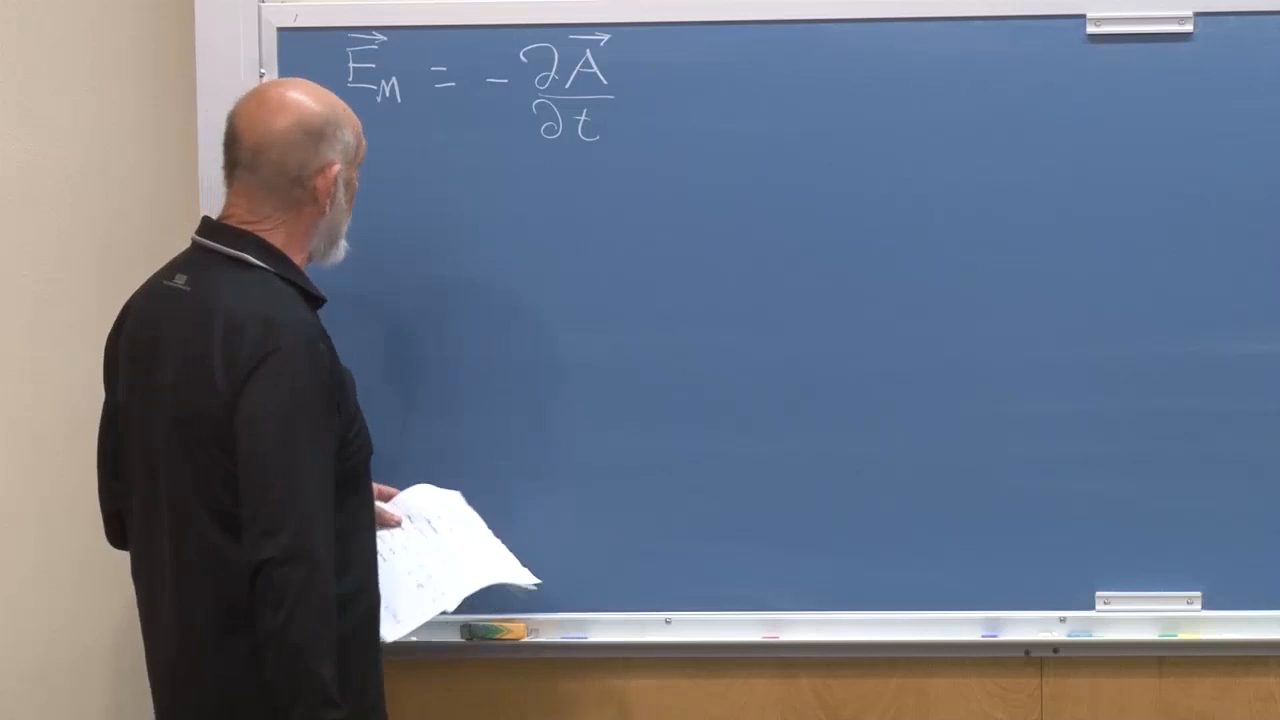
\includegraphics[width=\linewidth]{lecture_10_figure_02.png}\caption{El momento mecánico se introduce como la masa por la velocidad del centro de masas.}\par\smallskip
\textit{Fotograma de la lección: 00:11:15.}\end{figure}

\subsection{Momento canónico}

Supongamos que la mecánica se describe mediante \(L(q_i,\dot q_i)\). El momento canónico conjugado a \(q_i\) es \begin{equation}
p_i=\frac{\partial L}{\partial\dot q_i}.
\label{eq:canonical-momentum}
\end{equation}. Para \begin{equation}
L=\frac12 m\dot{\mathbf x}^{\,2}-V(\mathbf x),
\label{eq:simple-particle-lagrangian}
\end{equation}, esto da \(\mathbf p=m\dot{\mathbf x}\), de modo que, en este caso, el momento canónico y el mecánico coinciden.

\begin{figure}[H]\centering
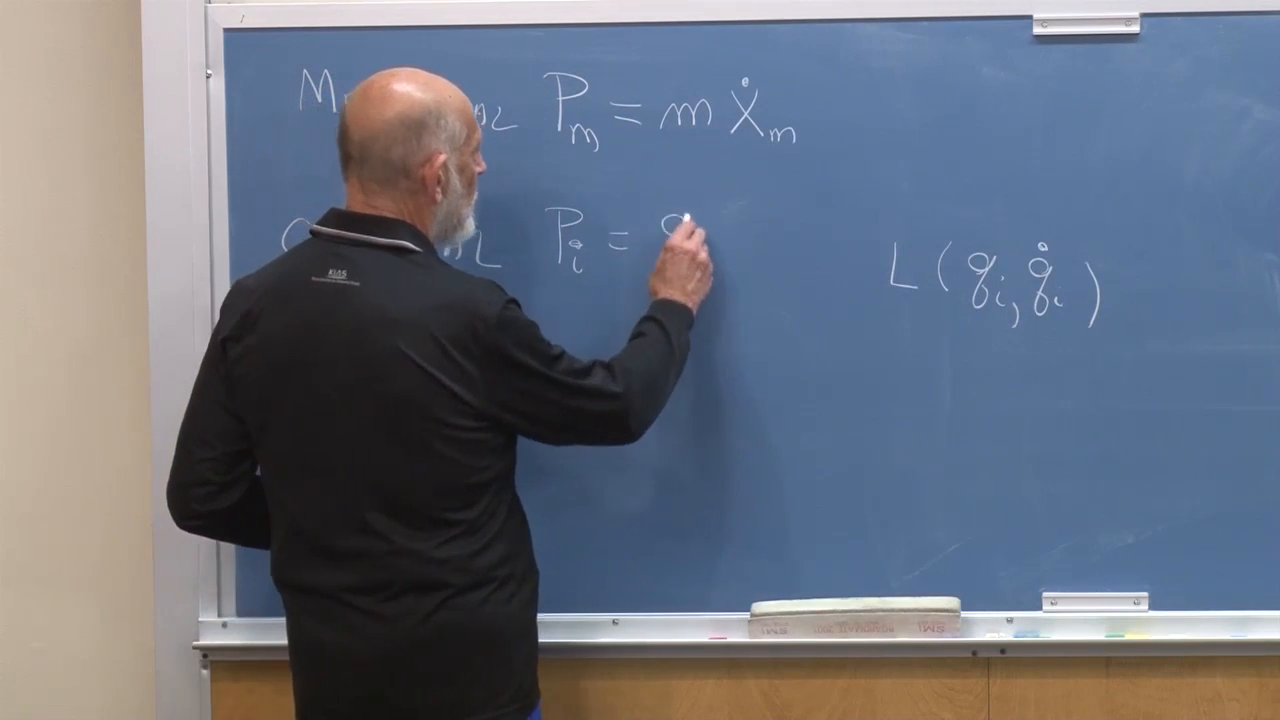
\includegraphics[width=\linewidth]{lecture_10_figure_03.png}\caption{El momento mecánico y el canónico junto a la lagrangiana de una partícula sencilla.}\par\smallskip
\textit{Fotograma de la lección: 00:13:40.}\end{figure}

Una partícula cargada en un campo magnético sirve de contraejemplo útil. Con la convención de signos escrita en la pizarra, \begin{equation}
L=\frac12m\dot{\mathbf x}^{\,2}-V(\mathbf x)
  -e\,\dot{\mathbf x}\cdot\mathbf A(\mathbf x),
\label{eq:magnetic-particle-lagrangian}
\end{equation}y, por tanto, \begin{equation}
p_i=m\dot x_i-eA_i.
\label{eq:magnetic-canonical-shift}
\end{equation}. Cambiar la convención de la carga o del término de interacción cambia el signo que aparece en la fórmula, pero no la conclusión: el momento canónico incluye una contribución del potencial vector y no es simplemente \(m\dot x_i\). Las ecuaciones de Hamilton usan la variable canónica. Más adelante se puede pasar el término dependiente del campo al otro lado de una ecuación y obtener una aceleración de aspecto newtoniano, pero esa reorganización no cambia la definición.

\begin{figure}[H]\centering
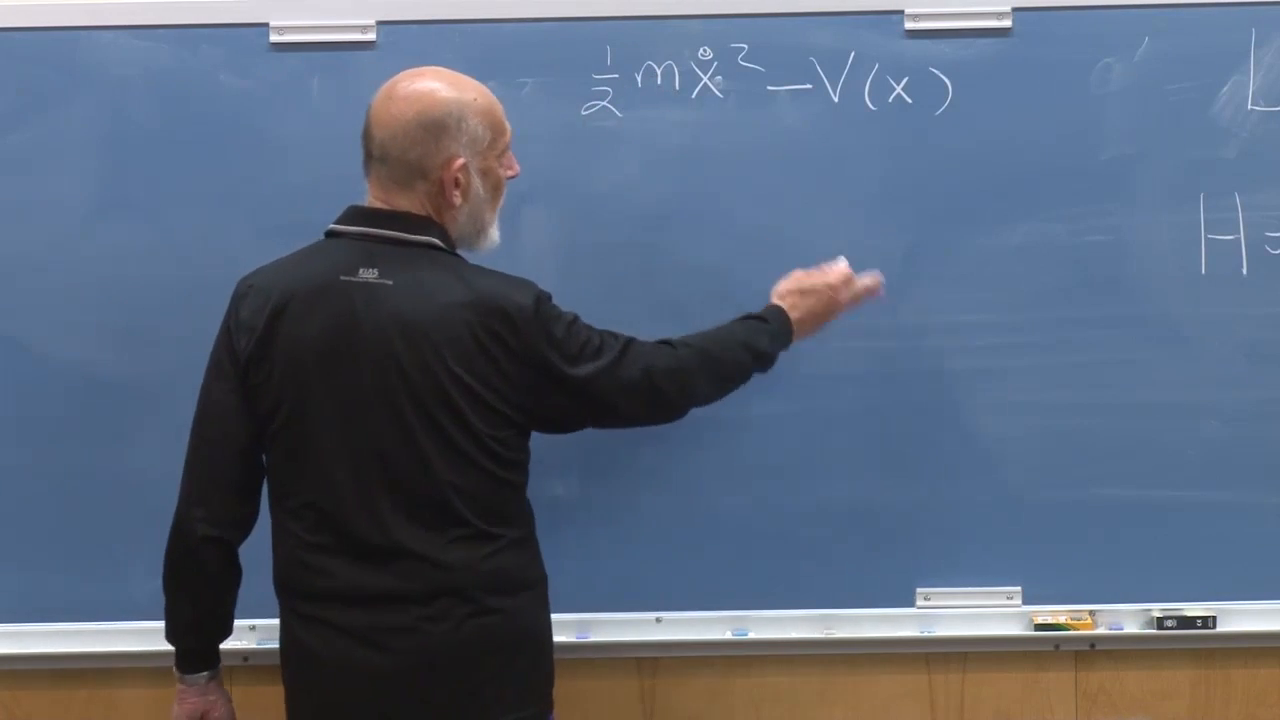
\includegraphics[width=\linewidth]{lecture_10_figure_04.png}\caption{El término del potencial vector desplaza el momento canónico con respecto al momento mecánico.}\par\smallskip
\textit{Fotograma de la lección: 00:15:50.}\end{figure}

\subsection{Momento de Noether}

El tercer momento es la carga conservada asociada a la invariancia bajo traslaciones espaciales. Para una simetría infinitesimal \begin{equation}
q_i\longrightarrow q_i+\delta q_i
\end{equation} que deja invariante la lagrangiana, el teorema de Noether da, salvo por la normalización del parámetro infinitesimal, \begin{equation}
Q=\sum_i p_i\,\delta q_i.
\label{eq:noether-charge-mechanics}
\end{equation}. Los \(p_i\) que aparecen aquí son momentos canónicos. Si la simetría es una traslación uniforme y el momento canónico coincide con el mecánico, \(Q\) se reduce al momento total habitual. En un sistema menos sencillo, esa coincidencia debe demostrarse, no darse por supuesta.

\begin{figure}[H]\centering
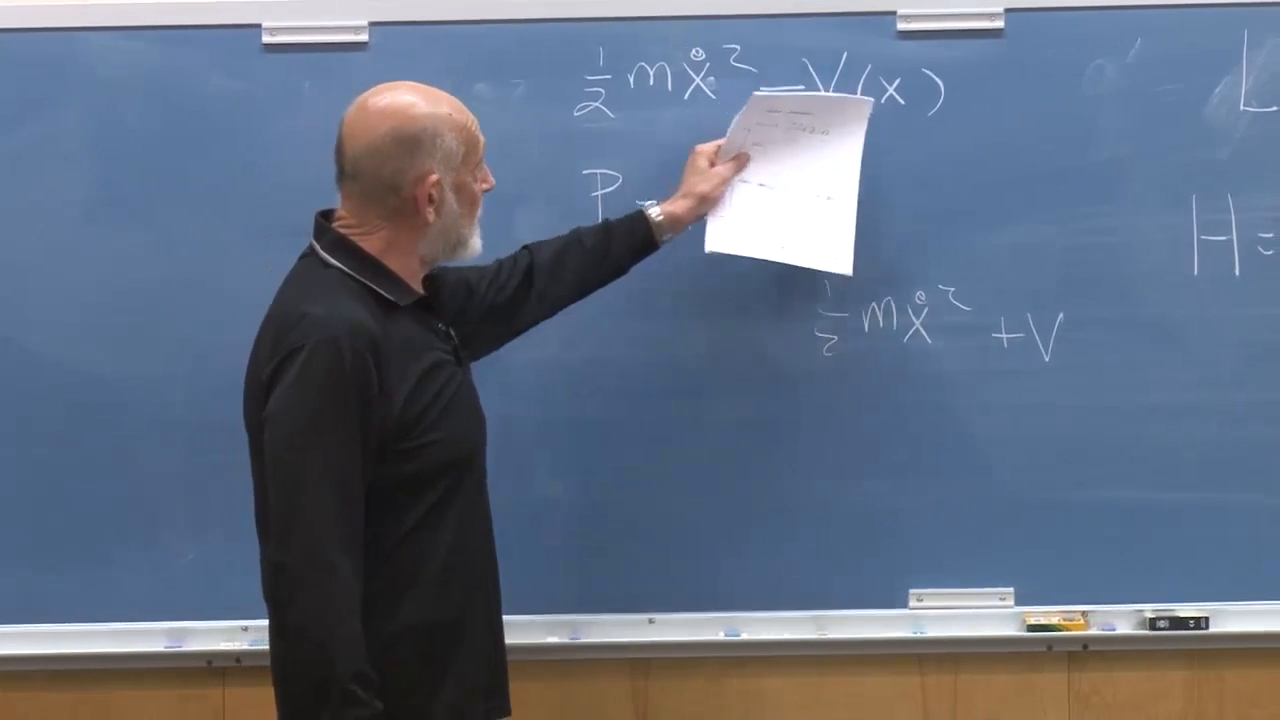
\includegraphics[width=\linewidth]{lecture_10_figure_05.png}\caption{La carga de Noether formada a partir de los momentos canónicos y las variaciones infinitesimales de las coordenadas.}\par\smallskip
\textit{Fotograma de la lección: 00:19:00.}\end{figure}

\section{La energía como hamiltoniano}

Las traslaciones espaciales conducen al momento; las traslaciones temporales, a la energía. Si la lagrangiana no depende explícitamente del tiempo, el hamiltoniano \begin{equation}
H=\sum_i p_i\dot q_i-L
\label{eq:hamiltonian-definition}
\end{equation} se conserva. Es la transformada de Legendre de la lagrangiana, no una regla para cambiar signos a simple vista.

\begin{figure}[H]\centering
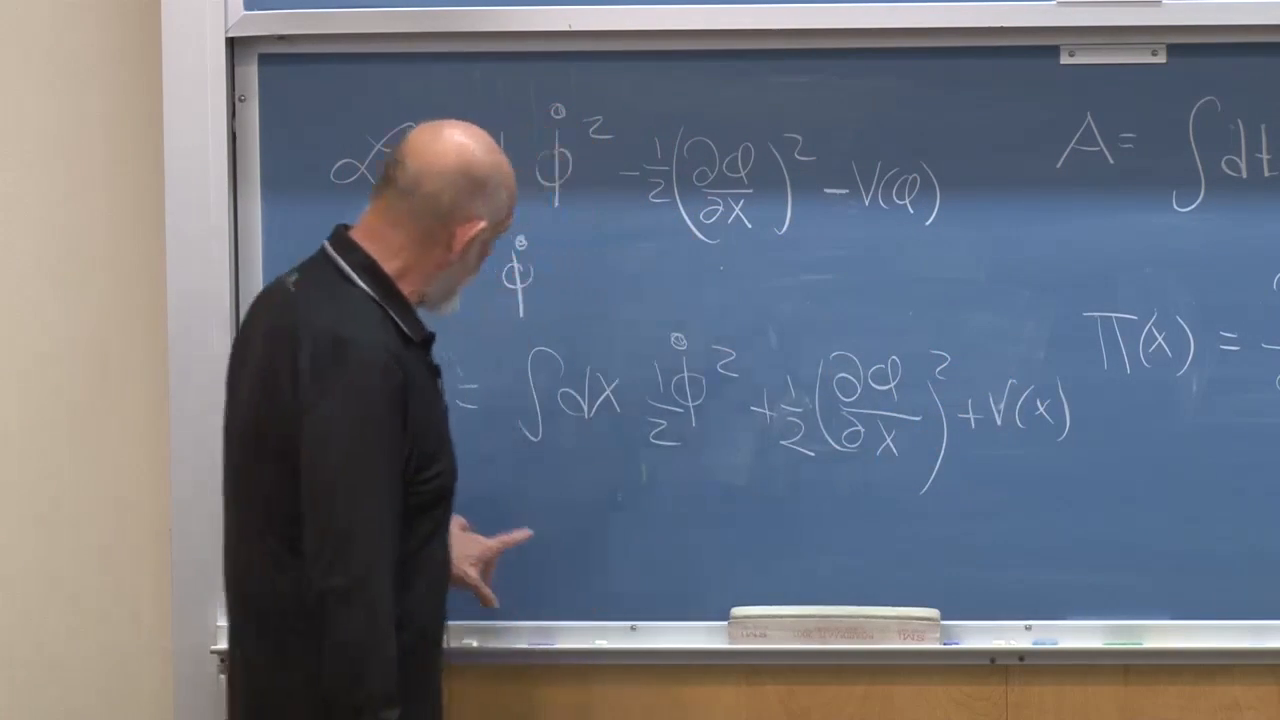
\includegraphics[width=\linewidth]{lecture_10_figure_06.png}\caption{El hamiltoniano expresado como la transformada de Legendre de una lagrangiana general.}\par\smallskip
\textit{Fotograma de la lección: 00:22:55.}\end{figure}

Para el ejemplo de una partícula, \begin{align}
p&=m\dot x,
\nonumber\\
H&=p\dot x-L\\
&=m\dot x^2
  -\left(\frac12m\dot x^2-V(x)\right)\\
&=\frac12m\dot x^2+V(x).
\label{eq:particle-hamiltonian}
\end{align}. Así, la lagrangiana es la energía cinética menos la energía potencial, mientras que el hamiltoniano es la energía cinética más la energía potencial.

\begin{figure}[H]\centering
\includegraphics[width=\linewidth]{lecture_10_figure_07.png}\caption{El cálculo para la partícula muestra cómo \(H=T+V\) se obtiene de \(H=p\dot x-L\).}\par\smallskip
\textit{Fotograma de la lección: 00:24:20.}\end{figure}

Cuando toda la dependencia de las velocidades consiste en términos cinéticos cuadráticos positivos convencionales y el resto no contiene velocidades, se puede obtener directamente el hamiltoniano cambiando el signo de la parte que no depende de las velocidades. Esta simplificación se usará repetidamente. Solo es válida porque, en los ejemplos considerados, la transformada de Legendre adopta esta forma sencilla.

\section{Un campo es un sistema mecánico con un continuo de coordenadas}

Para poner de manifiesto la estructura mecánica de la teoría de campos, elijamos un sistema inercial y dejemos temporalmente de exigir que cada línea muestre la covariancia de Lorentz de forma manifiesta. La mecánica clásica tiene un eje temporal y coordenadas \(q_i(t)\). Un campo escalar tiene un eje temporal y coordenadas \(\phi(\mathbf x,t)\). La etiqueta discreta \(i\) simplemente se ha convertido en la etiqueta continua \(\mathbf x\): \begin{equation}
q_i(t)\quad\longrightarrow\quad\phi(\mathbf x,t).
\label{eq:discrete-to-field}
\end{equation}. El valor del campo en cada punto espacial constituye un grado de libertad. Aquí, \(\mathbf x\) indica de qué grado de libertad se trata; no es en sí misma la coordenada generalizada.

\begin{figure}[H]\centering
\includegraphics[width=\linewidth]{lecture_10_figure_08.png}\caption{Una red espacial que muestra el valor del campo en cada punto como un grado de libertad mecánico independiente.}\par\smallskip
\textit{Fotograma de la lección: 00:30:15.}\end{figure}

\begin{classroomqa}\audiencequestion{¿Por qué no escribir el campo como \(\phi(\mathbf x,t)\) desde el principio?}\lecturerresponse{Esa es la notación completa. La expresión temporal \(\phi(\mathbf x)\) omite el argumento temporal común, igual que a menudo se escribe \(q_i\) teniendo presente que cada \(q_i\) depende del tiempo. La etiqueta \(i\), o ahora \(\mathbf x\), nos indica qué grado de libertad estamos considerando. \lecturetimestamp{00:32:43}}\end{classroomqa}

\begin{classroomqa}
\audiencequestion{¿Son realmente independientes las coordenadas que representan los valores del campo en puntos vecinos? ¿Qué impone la continuidad?}
\lecturerresponse{Son coordenadas canónicas independientes. La suavidad no se impone identificando los valores vecinos, sino que se selecciona dinámicamente. El hamiltoniano contiene un término positivo de energía del gradiente, por lo que mantener un salto fijo a lo largo de una distancia cada vez menor cuesta cada vez más energía. En consecuencia, las configuraciones de energía finita son suaves en el límite continuo. \lecturetimestamp{00:33:09}}\end{classroomqa}

Una derivada espacial hace explícito el acoplamiento entre grados de libertad vecinos. En una red de espaciado \(\epsilon\), \begin{equation}
\partial_x\phi(x,t)
  =\lim_{\epsilon\to0}
   \frac{\phi(x+\epsilon,t)-\phi(x,t)}{\epsilon}.
\label{eq:field-finite-difference}
\end{equation}. Depende de dos coordenadas próximas, pero no contiene ninguna velocidad generalizada. En la analogía mecánica pertenece a la dependencia de la lagrangiana respecto de las coordenadas, no a la dependencia respecto de \(\dot q_i\).

\begin{figure}[H]\centering
\includegraphics[width=\linewidth]{lecture_10_figure_09.png}\caption{La derivada espacial reconstruida como una diferencia entre valores del campo en puntos vecinos de la red.}\par\smallskip
\textit{Fotograma de la lección: 00:31:40.}\end{figure}

Ahora se puede escribir la acción de forma explícitamente mecánica: \begin{align}
S&=\int dt\,L,
\nonumber\\
L&=\int d^3x\,
\mathcal L\!\left(
\phi,\dot\phi,\boldsymbol{\nabla}\phi
\right),
\nonumber\\
S&=\int dt\,d^3x\,
\mathcal L\!\left(
\phi,\dot\phi,\boldsymbol{\nabla}\phi
\right).
\label{eq:field-action-split}
\end{align}. La letra caligráfica \(\mathcal L\) representa la densidad lagrangiana; al integrarla en el espacio se obtiene la lagrangiana ordinaria, que se integra a su vez en el tiempo. Una teoría local acopla cada punto únicamente mediante los campos y sus derivadas en ese mismo punto. Separar el tiempo del espacio oculta momentáneamente la covariancia de Lorentz, pero hace transparente la mecánica.

\begin{figure}[H]\centering
\includegraphics[width=\linewidth]{lecture_10_figure_10.png}\caption{La acción del campo separada en una integral temporal y una integral espacial de la densidad lagrangiana.}\par\smallskip
\textit{Fotograma de la lección: 00:36:40.}\end{figure}

\section{Momento canónico de campo y densidad hamiltoniana}

La velocidad de una coordenada de campo es \(\dot\phi(\mathbf x,t)\): la tasa de cambio temporal del campo en un punto fijo. No es movimiento de un punto espacial a otro. Por tanto, el momento canónico conjugado al campo es, a su vez, un campo: \begin{equation}
\Pi(\mathbf x,t)
 =\frac{\partial\mathcal L}{\partial\dot\phi(\mathbf x,t)}.
\label{eq:field-canonical-momentum}
\end{equation}. Para varios campos \(\phi_a\), hay un campo de momento \(\Pi_a\) para cada uno.

La suma discreta de la transformada de Legendre se convierte en una integral espacial: \begin{align}
H
 &=\int d^3x\,
   \left[\Pi\dot\phi-\mathcal L\right]
  =\int d^3x\,\mathcal H,
\nonumber\\
\mathcal H
 &=\Pi\dot\phi-\mathcal L .
\label{eq:field-hamiltonian-density}
\end{align}. La cantidad que aparece dentro de la integral es la densidad de energía.

\begin{figure}[H]\centering
\includegraphics[width=\linewidth]{lecture_10_figure_11.png}\caption{La transformada de Legendre del campo y su interpretación como integral de la densidad local de energía.}\par\smallskip
\textit{Fotograma de la lección: 00:42:40.}\end{figure}

\begin{classroomqa}\audiencequestion{¿Por qué puede sustituirse la derivada de la lagrangiana total respecto de \(\dot\phi\) en un punto por la derivada de la densidad local allí?}\lecturerresponse{Piénsese en la integral espacial como una suma continua. Bajo el supuesto de localidad usado aquí, la velocidad \(\dot\phi(\mathbf x)\) solo aparece en el término correspondiente a ese mismo punto. Al derivar respecto de esa velocidad concreta, todos los demás términos desaparecen. Las derivadas espaciales pueden acoplar valores del campo en puntos vecinos, pero en esta teoría no introducen derivadas temporales en puntos vecinos. \lecturetimestamp{00:51:56}}\end{classroomqa}

\subsection{El campo escalar}

En una dimensión espacial, tomemos \begin{equation}
\mathcal L
 =\frac12\dot\phi^2
  -\frac12(\partial_x\phi)^2
  -V(\phi).
\label{eq:scalar-field-lagrangian}
\end{equation}. Esta es la expresión no covariante del escalar de Lorentz usado antes: el signo menos relativo entre las derivadas temporales y espaciales proviene de la métrica de Minkowski. El momento canónico es \begin{equation}
\Pi=\dot\phi,
\label{eq:scalar-pi}
\end{equation} y el hamiltoniano queda \begin{equation}
H=\int dx\,
\left[
\frac12\dot\phi^2
+\frac12(\partial_x\phi)^2
+V(\phi)
\right].
\label{eq:scalar-field-hamiltonian}
\end{equation}. Durante el cálculo, se llamó por un momento \(V(x)\) al potencial; la clase corrigió la expresión a \(V(\phi)\). Puede depender indirectamente de la posición a través del campo, pero en la teoría invariante bajo traslaciones no tiene una dependencia externa prescrita respecto de \(x\).

\begin{figure}[H]\centering
\includegraphics[width=\linewidth]{lecture_10_figure_12.png}\caption{La densidad lagrangiana escalar, el momento conjugado y el hamiltoniano positivo reunidos en una misma pizarra.}\par\smallskip
\textit{Fotograma de la lección: 00:47:05.}\end{figure}

Toda la parte que no contiene derivadas temporales desempeña el papel de energía potencial. Esto incluye tanto \(V(\phi)\) como la energía del gradiente \(\frac12(\partial_x\phi)^2\). La lagrangiana puede tener cualquiera de los dos signos; la energía de un sistema estable debe estar acotada inferiormente.

\begin{classroomqa}\audiencequestion{¿Puede ser negativo el potencial \(V(\phi)\)}\lecturerresponse{Sí. Si tiene una cota inferior finita, se le puede sumar una constante para que su mínimo sea cero sin cambiar la ecuación clásica del campo. Un potencial no acotado inferiormente describe una inestabilidad: el campo puede reducir su energía sin límite. El vacío estable es un campo constante situado en un mínimo del potencial desplazado. \lecturetimestamp{00:49:03}}\end{classroomqa}

Ahora se puede responder cuantitativamente a la pregunta anterior sobre la continuidad. Un salto \(\Delta\phi\) a través de un espaciado de red \(\epsilon\) contribuye \begin{equation}
\frac12(\partial_x\phi)^2
\sim\frac12\left(\frac{\Delta\phi}{\epsilon}\right)^2.
\label{eq:gradient-cost}
\end{equation}. Cuando \(\epsilon\to0\), un salto fijo da lugar a una densidad de energía arbitrariamente grande. Por tanto, la energía finita suprime las configuraciones irregulares.

\begin{figure}[H]\centering
\includegraphics[width=\linewidth]{lecture_10_figure_13.png}\caption{La fórmula de la energía del campo escalar se conserva mientras el dibujo en la pizarra compara un campo suave con una variación brusca.}\par\smallskip
\textit{Fotograma de la lección: 00:54:20.}\end{figure}

\section{Energía local y significado de \texorpdfstring{\(T^{00}\)}{T00}}

La densidad de energía recibe un nombre compacto: \begin{equation}
T^{00}=\mathcal H=\Pi\dot\phi-\mathcal L.
\label{eq:T00-definition}
\end{equation}. Los dos índices nulos codifican dos afirmaciones distintas. La energía es la componente temporal \(P^0\) del cuadrivector de energía--momento, mientras que una densidad es la componente temporal de una corriente conservada. Así pues, \(T^{00}\) es la densidad de la componente temporal del cuadrimomento.

\begin{figure}[H]\centering
\includegraphics[width=\linewidth]{lecture_10_figure_14.png}\caption{La energía del campo escrita localmente e identificada con \(T^{00}\).}\par\smallskip
\textit{Fotograma de la lección: 01:00:00.}\end{figure}

En una teoría relativista local, la conservación no consiste únicamente en afirmar que una cantidad global permanece invariable. La energía no puede desaparecer en el laboratorio y reaparecer en Alfa Centauri. Todo cambio dentro de una región debe explicarse mediante un flujo a través de su frontera. En forma local, \begin{equation}
\partial_\mu T^{\mu\nu}=0,
\label{eq:stress-energy-continuity}
\end{equation}; por tanto, el primer índice indica la densidad o la dirección del flujo, y el segundo indica qué componente \(P^\nu\) se transporta.

\begin{classroomqa}\audiencequestion{¿Decir que \(T^{00}\) es una densidad significa que la energía total se obtiene integrándola?}\lecturerresponse{Exactamente: \(E=P^0=\int d^3x\,T^{00}\). La densidad local es el integrando de la transformada de Legendre del campo. Una variación suya en un lugar se compensa mediante una corriente de energía entre puntos vecinos. \lecturetimestamp{00:59:06}}\end{classroomqa}

\section{Densidad de momento a partir de las traslaciones espaciales}

Volvamos a la fórmula de Noether, sustituyendo ahora la suma discreta por una integral espacial. Bajo una pequeña traslación en la dirección \(m\), el campo cambia en \begin{equation}
\delta\phi
  =\phi(\mathbf x)-\phi(\mathbf x-\boldsymbol{\epsilon})
  =\epsilon^m\partial_m\phi+O(\epsilon^2),
\label{eq:translated-field-change}
\end{equation}, según la convención pasiva usada en la pizarra. Invertir las traslaciones activas y pasivas invierte el signo global; una vez elegida esa convención, queda fijado el generador físico. Al factorizar \(\epsilon^m\), el momento de Noether tiene la estructura \begin{equation}
P_m\ \propto\ \int d^3x\,\Pi\,\partial_m\phi.
\label{eq:scalar-noether-momentum}
\end{equation}.

\begin{figure}[H]\centering
\includegraphics[width=\linewidth]{lecture_10_figure_15.png}\caption{Un perfil de campo trasladado y la derivada que mide su cambio infinitesimal.}\par\smallskip
\textit{Fotograma de la lección: 01:04:20.}\end{figure}

\begin{classroomqa}\audiencequestion{¿Por qué no se mantuvo la traslación infinitesimal \(\epsilon\) en la fórmula del momento?}\lecturerresponse{La carga de Noether se obtiene primero como una cantidad proporcional a \(\epsilon\). El momento se define como el coeficiente de ese parámetro de traslación arbitrario, así que se divide por \(\epsilon\). Multiplicar una cantidad conservada por una constante fija no alteraría su conservación, pero extraer el coeficiente proporciona la normalización estándar. \lecturetimestamp{01:04:45}}\end{classroomqa}

\begin{classroomqa}\audiencequestion{¿El intervalo de traslación se convierte en \(dx\) en la integral continua?}\lecturerresponse{Proceden de límites distintos. La medida \(dx\) aparece al sustituir la suma sobre los grados de libertad etiquetados espacialmente por una integral. El parámetro de traslación \(\epsilon\) describe la operación de simetría y se factoriza en la carga de Noether correspondiente. Ambos son infinitesimales en el razonamiento intermedio, pero cumplen funciones distintas. \lecturetimestamp{01:05:16}}\end{classroomqa}

En la notación de la lección, la densidad de la componente \(m\) del momento es \begin{equation}
T^{0m}=\Pi\,\partial_m\phi,
\label{eq:scalar-momentum-density}
\end{equation}, con la convención de signos de traslación sobrentendida. Para la teoría escalar \(\Pi=\dot\phi\), de modo que es proporcional a \(\dot\phi\,\partial_m\phi\).

\begin{figure}[H]\centering
\includegraphics[width=\linewidth]{lecture_10_figure_16.png}\caption{La densidad de momento de Noether \(T^{0m}=\Pi\,\partial_m\phi\) en la pizarra.}\par\smallskip
\textit{Fotograma de la lección: 01:07:10.}\end{figure}

Este es el momento literal transportado por una onda. La invariancia bajo traslaciones solo se aplica cuando se traslada todo: campos, partículas, fuentes y aparatos. Un pulso de luz absorbido por una placa suspendida libremente le comunica un retroceso. La luz ordinaria produce un efecto diminuto; un láser lo bastante potente puede transferir suficiente momento para comprimir un blanco pequeño. La cantidad total conservada corresponde conjuntamente a las partículas y los campos.

\subsection{¿Qué sustituye a la ecuación de Newton?}

La ecuación de Euler--Lagrange del campo, deducida de la ec.~\eqref{eq:scalar-field-lagrangian}, es \begin{equation}
\ddot\phi-\nabla^2\phi=-\frac{dV}{d\phi}.
\label{eq:scalar-equation-of-motion}
\end{equation}. Es la análoga de la ley de Newton en la teoría de campos.

\begin{figure}[H]\centering
\includegraphics[width=\linewidth]{lecture_10_figure_17.png}\caption{La ecuación del campo escalar junto a su hamiltoniano y su densidad de momento.}\par\smallskip
\textit{Fotograma de la lección: 01:12:55.}\end{figure}

\begin{classroomqa}\audiencequestion{¿Qué corresponde a la ley de Newton para un campo?}\lecturerresponse{La ecuación de Euler--Lagrange del campo. Aquí es una ecuación de onda con el término de fuerza \(-V'(\phi)\). El papel de \(m\ddot x=-V'(x)\) lo desempeña \(\ddot\phi-\nabla^2\phi=-V'(\phi)\). \lecturetimestamp{01:11:48}}\end{classroomqa}

\begin{classroomqa}\audiencequestion{¿Cómo sabemos si una lagrangiana de campo propuesta es correcta? ¿Hay que conocer ya la ecuación del campo?}\lecturerresponse{Se puede proceder en cualquiera de los dos sentidos. Históricamente, se pueden inferir ecuaciones a partir de experimentos y luego buscar una acción, como ocurrió con Newton y Maxwell. En la teoría moderna, a menudo se parte del contenido de campos, la localidad, la simetría y un pequeño conjunto de términos admisibles; se deducen las ecuaciones y se ponen a prueba sus predicciones. El escalar mostrado podría describir un campo fundamental, pero también podría describir el desplazamiento transversal de una cuerda, cuya acción continua se deduce de las partículas que la constituyen. \lecturetimestamp{01:12:55}}\end{classroomqa}

\section{El campo electromagnético en el gauge temporal}

Las componentes que ya se han obtenido, \(T^{00}\) y \(T^{0m}\), pertenecen al tensor de energía--momento. Sus componentes restantes describen los flujos de energía y momento. Más adelante, este tensor será fuente de gravedad, pero el electromagnetismo ofrece un ejemplo inmediato.

La coordenada electromagnética básica es el cuadripotencial \(A_\mu\). La libertad de gauge permite \begin{equation}
A_\mu\longrightarrow A'_\mu=A_\mu+\partial_\mu S
\label{eq:gauge-transformation-lecture10}
\end{equation} sin cambiar \(F_{\mu\nu}\). Elijamos \(S\) de modo que satisfaga \begin{equation}
\partial_tS=-A_0.
\label{eq:temporal-gauge-choice}
\end{equation}. Por ejemplo, se puede integrar \(A_0\) respecto del tiempo en cada punto espacial fijo. La componente temporal transformada se anula entonces: \begin{equation}
A'_0=A_0+\partial_tS=0.
\label{eq:temporal-gauge}
\end{equation}. Este es el gauge temporal. Elimina \(A_0\) de la lista de coordenadas dinámicas, aunque la ley de Gauss sigue siendo una restricción y persiste una libertad de gauge residual independiente del tiempo.

\begin{figure}[H]\centering
\includegraphics[width=\linewidth]{lecture_10_figure_18.png}\caption{Libertad de gauge usada para elegir \(A_0=0\) resolviendo \(\partial_tS=-A_0\).}\par\smallskip
\textit{Fotograma de la lección: 01:20:15.}\end{figure}

A partir de aquí, sea \(\mathbf E\) el campo estándar de Maxwell. Antes de fijar el gauge, \begin{equation}
E_m=-\partial_tA_m+\partial_mA_0,
\qquad
\mathbf B=\boldsymbol{\nabla}\times\mathbf A.
\label{eq:E-B-general-potential}
\end{equation}. En el gauge temporal, estas expresiones se reducen a \begin{equation}
\mathbf E=-\dot{\mathbf A},
\qquad
\mathbf B=\boldsymbol{\nabla}\times\mathbf A.
\label{eq:E-B-temporal-gauge}
\end{equation}. Las derivadas temporales de \(\mathbf A\) producen el campo eléctrico; las derivadas espaciales producen el campo magnético.

\begin{figure}[H]\centering
\includegraphics[width=\linewidth]{lecture_10_figure_19.png}\caption{Los campos eléctrico y magnético en el gauge temporal: \(\mathbf E=-\dot{\mathbf A}\) y \(\mathbf B=\nabla\times\mathbf A\).}\par\smallskip
\textit{Fotograma de la lección: 01:23:50.}\end{figure}

\section{Momento canónico y energía electromagnéticos}

La densidad lagrangiana de Maxwell en el vacío es \begin{equation}
\mathcal L_{\mathrm{EM}}
 =-\frac14F_{\mu\nu}F^{\mu\nu}
 =\frac12\left(\mathbf E^2-\mathbf B^2\right).
\label{eq:maxwell-lagrangian-energy-lecture}
\end{equation}. En el gauge temporal, \begin{equation}
\mathcal L_{\mathrm{EM}}
 =\frac12\dot{\mathbf A}^{\,2}
  -\frac12(\boldsymbol{\nabla}\times\mathbf A)^2.
\label{eq:maxwell-lagrangian-temporal}
\end{equation}. Tiene exactamente la estructura del campo escalar: cuadrados de derivadas temporales menos cuadrados de derivadas espaciales.

\begin{figure}[H]\centering
\includegraphics[width=\linewidth]{lecture_10_figure_20.png}\caption{La lagrangiana de Maxwell reescrita como lagrangiana mecánica de campo para las componentes espaciales de \(\mathbf A\).}\par\smallskip
\textit{Fotograma de la lección: 01:28:10.}\end{figure}

Cada componente \(A_m\) tiene un momento canónico: \begin{equation}
\Pi_m
 =\frac{\partial\mathcal L_{\mathrm{EM}}}
        {\partial\dot A_m}
 =\dot A_m
 =-E_m.
\label{eq:em-canonical-momentum}
\end{equation}. Este es un ejemplo concreto de por qué importa la convención. Con la convención opuesta para el campo eléctrico usada antes, cambiaría el signo final que se muestra, aunque la propia derivada canónica no cambiaría.

\begin{figure}[H]\centering
\includegraphics[width=\linewidth]{lecture_10_figure_21.png}\caption{Los tres campos de momento canónico asociados a \(A_x,A_y,A_z\), cada uno igual a la derivada temporal correspondiente y, por tanto, al negativo del campo eléctrico estándar.}\par\smallskip
\textit{Fotograma de la lección: 01:30:20.}\end{figure}

Ahora queda justificada la simplificación para obtener el hamiltoniano: se cambia el signo del término que no contiene derivadas temporales. La densidad de energía electromagnética es \begin{equation}
T^{00}_{\mathrm{EM}}
 =\mathcal H_{\mathrm{EM}}
 =\frac12\left(\mathbf E^2+\mathbf B^2\right),
\label{eq:em-energy-density}
\end{equation} y \begin{equation}
H_{\mathrm{EM}}
 =\int d^3x\,
\frac12\left(\mathbf E^2+\mathbf B^2\right).
\label{eq:em-total-energy}
\end{equation}. A diferencia de la densidad lagrangiana, la densidad de energía es no negativa.

\begin{figure}[H]\centering
\includegraphics[width=\linewidth]{lecture_10_figure_22.png}\caption{La densidad hamiltoniana electromagnética positiva \(\frac12(\mathbf E^2+\mathbf B^2)\).}\par\smallskip
\textit{Fotograma de la lección: 01:32:00.}\end{figure}

Para una onda plana en el vacío, \(\mathbf E\perp\mathbf B\), los dos campos están en fase y, en unidades \(c=1\), tienen la misma magnitud. Por tanto, las contribuciones eléctrica y magnética se reparten por igual la energía de la onda: \begin{equation}
u_E=\frac12\mathbf E^2,
\qquad
u_B=\frac12\mathbf B^2,
\qquad
u_E=u_B.
\label{eq:plane-wave-energy-halves}
\end{equation}.

\section{Deducción del momento electromagnético}

Ahora hay que sumar la fórmula de traslación de Noether sobre los tres campos \(A_m\). Si se elige el signo de la traslación de modo que el momento físico apunte en la dirección de propagación de la onda, la componente \(n\) es \begin{equation}
P_n
 =\int d^3x\,E_m\,\partial_nA_m,
\label{eq:em-canonical-noether-momentum}
\end{equation}, donde se suma sobre \(m\). La lección se detiene deliberadamente en el signo: depende de las elecciones anteriores para el campo eléctrico y para las traslaciones activas o pasivas. El resultado físico, invariante bajo transformaciones de gauge, lo fijará.

\begin{figure}[H]\centering
\includegraphics[width=\linewidth]{lecture_10_figure_23.png}\caption{La fórmula de Noether para el campo escalar extendida a las tres componentes del potencial vector.}\par\smallskip
\textit{Fotograma de la lección: 01:36:40.}\end{figure}

El integrando todavía contiene el potencial de gauge, no solo los campos físicos. Sumemos y restemos \(E_m\partial_mA_n\): \begin{align}
E_m\partial_nA_m
 &=
 E_m\left(\partial_nA_m-\partial_mA_n\right)
 +E_m\partial_mA_n.
\label{eq:add-subtract-em-momentum}
\end{align}. El primer término es un producto vectorial: \begin{equation}
E_m\left(\partial_nA_m-\partial_mA_n\right)
  =(\mathbf E\times\mathbf B)_n.
\label{eq:cross-product-component}
\end{equation}. El segundo se integra por partes: \begin{align}
\int d^3x\,E_m\partial_mA_n
 &=
\int_{\partial V}d\Sigma_m\,E_mA_n
-\int d^3x\,A_n\partial_mE_m.
\label{eq:em-momentum-integration-parts}
\end{align}. Si los campos decrecen de modo que el término de frontera se anule y la región no contiene fuentes, de manera que \(\boldsymbol{\nabla}\cdot\mathbf E=0\), el segundo término no aporta nada.

\begin{figure}[H]\centering
\includegraphics[width=\linewidth]{lecture_10_figure_24.png}\caption{El término añadido trasladado a \(\nabla\cdot\mathbf E\) mediante integración por partes.}\par\smallskip
\textit{Fotograma de la lección: 01:40:00.}\end{figure}

Por tanto, el momento total del campo es \begin{equation}
\mathbf P_{\mathrm{EM}}
 =\int d^3x\,\mathbf E\times\mathbf B,
\qquad
\mathbf g_{\mathrm{EM}}
 =\mathbf E\times\mathbf B,
\label{eq:em-momentum-density}
\end{equation} en las unidades de la lección. El vector \(\mathbf g_{\mathrm{EM}}\) es la densidad de momento electromagnética.

\begin{figure}[H]\centering
\includegraphics[width=\linewidth]{lecture_10_figure_25.png}\caption{La expresión con el potencial de gauge reducida al momento invariante bajo transformaciones de gauge \(\int d^3x\,\mathbf E\times\mathbf B\).}\par\smallskip
\textit{Fotograma de la lección: 01:41:10.}\end{figure}

\begin{classroomqa}\audiencequestion{¿Dónde se usó \(\boldsymbol{\nabla}\cdot\mathbf E=0\) y qué ocurre si hay cargas?}\lecturerresponse{Permite eliminar el término de volumen tras integrar por partes, de modo que la deducción mostrada, basada solo en el campo, se aplica a una onda electromagnética libre. Si hay carga, ese término no se anula y hay que incluir el momento de la materia cargada. La invariancia bajo traslaciones y la conservación del momento conciernen al sistema completo de materia--campo. \lecturetimestamp{01:41:55}}\end{classroomqa}

\subsection{Dirección del momento de la onda}

En una onda plana, \(\mathbf E\), \(\mathbf B\) y la dirección de propagación forman una terna dextrógira. Media longitud de onda después, tanto \(\mathbf E\) como \(\mathbf B\) se invierten: \begin{equation}
(-\mathbf E)\times(-\mathbf B)
 =\mathbf E\times\mathbf B.
\label{eq:poynting-sign-reversal}
\end{equation}. Por tanto, la densidad de momento apunta en todo momento de la oscilación en una misma dirección: la de propagación de la onda.

\begin{figure}[H]\centering
\includegraphics[width=\linewidth]{lecture_10_figure_26.png}\caption{Geometría de la onda plana: los campos eléctrico y magnético se invierten juntos, mientras que su producto vectorial sigue apuntando a lo largo del eje de propagación.}\par\smallskip
\textit{Fotograma de la lección: 01:43:10.}\end{figure}

Por eso la presión de la luz es real. La absorción transfiere el momento del campo a la materia; la reflexión invierte el momento de la luz y puede transferir al reflector el doble de la componente normal.

\section{Donde el potencial se relaciona con los campos observables}

Al final, la clase pregunta cómo se relaciona \(A_\mu\) con los campos observables. La relación es exactamente
\begin{align}
E_n&=-\partial_tA_n+\partial_nA_0,
\nonumber\\
B_n&=\epsilon_{nmk}\partial_mA_k.
\label{eq:potential-field-contact}
\end{align}
El gauge temporal elimina el término \(A_0\), pero no cambia los campos físicos.

\begin{figure}[H]
\centering
\includegraphics[width=\linewidth]{lecture_10_figure_27.png}
\caption{Relación general del campo eléctrico, recuperada tras el cálculo en gauge temporal, junto con el lagrangiano escalar covariante que se recuerda debajo.}
\par\smallskip
\textit{Fotograma de la clase: 01:45:40.}
\end{figure}

\begin{classroomqa}
\audiencequestion{¿Dónde se relacionan exactamente el potencial vector y los campos eléctrico y magnético?}
\lecturerresponse{El campo eléctrico combina la derivada temporal del potencial espacial con la derivada espacial de \(A_0\); el campo magnético es el rotacional del potencial espacial. En gauge temporal, esto se reduce simplemente a
\(\mathbf E=-\dot{\mathbf A}\) y
\(\mathbf B=\nabla\times\mathbf A\).
\lecturetimestamp{01:44:15}}
\end{classroomqa}

\begin{classroomqa}
\audiencequestion{¿Es el potencial más fundamental que \(\mathbf E\) y \(\mathbf B\)?}
\lecturerresponse{La acción y el principio de gauge se formulan de la manera más natural en términos de \(A_\mu\), lo que confiere al potencial un carácter fundamental en la estructura de la teoría. Sin embargo, \(A_\mu\) no es único: los potenciales relacionados por una transformación de gauge representan la misma física, y los campos locales son invariantes gauge. Ambas afirmaciones son compatibles. Las variables fundamentales no tienen por qué ser directamente observables. \lecturetimestamp{01:46:36}}
\end{classroomqa}

\begin{classroomqa}
\audiencequestion{¿Puede el potencial de gauge por sí mismo ejercer una fuerza?}
\lecturerresponse{Una representación dependiente del gauge no puede producir una fuerza medible que dependa del gauge. La materia cargada se acopla mediante el potencial en la acción, pero la fuerza de Lorentz clásica puede expresarse enteramente en términos de los campos eléctrico y magnético, que son invariantes gauge.
\lecturetimestamp{01:47:49}}
\end{classroomqa}

\begin{classroomqa}
\audiencequestion{Si los campos eléctrico y magnético cruzados son estáticos, ¿su momento debe ser cero?}
\lecturerresponse{No necesariamente para el campo por sí solo:
\(\mathbf E\times\mathbf B\) puede ser distinto de cero incluso cuando ambos campos son independientes del tiempo. En un dispositivo estático cerrado, el balance total del momento también incluye las cargas, las corrientes, los soportes y cualquier momento mecánico u oculto. La breve respuesta dada en clase —que el total debe equilibrarse— es la afirmación correcta de conservación; imponer que la contribución del campo por sí sola sea cero sería ir demasiado lejos.
\lecturetimestamp{01:48:01}}
\end{classroomqa}

\section{Un tensor, dos significados del vector de Poynting}

El tensor de energía--momento organiza todas las densidades y los flujos:
\begin{align}
T^{00}&=\text{energy density},\\
T^{0i}&=\text{\(i\)-momentum density},\\
T^{i0}&=\text{energy flux in the \(i\)-direction},\\
T^{ij}&=\text{\(j\)-momentum flux in the \(i\)-direction}.
\label{eq:stress-energy-components}
\end{align}
Por ejemplo, \(T^{31}\) es la cantidad de momento en la dirección \(x\) que atraviesa, por unidad de tiempo, una unidad de área cuya normal apunta en la dirección \(z\). El bloque espacial \(T^{ij}\) es el tensor de esfuerzos.

\begin{figure}[H]
\centering
\includegraphics[width=\linewidth]{lecture_10_figure_28.png}
\caption{En la pizarra se empieza a organizar las componentes de densidad y flujo en el tensor de energía--momento.}
\par\smallskip
\textit{Fotograma de la clase: 01:51:10.}
\end{figure}

Para los sistemas relativistas que estamos considerando, se puede elegir simétrico el tensor físico de energía--momento:
\begin{equation}
T^{\mu\nu}=T^{\nu\mu}.
\label{eq:stress-energy-symmetry}
\end{equation}
Por consiguiente,
\begin{equation}
T^{0i}=T^{i0}.
\label{eq:momentum-density-energy-flux}
\end{equation}
La densidad de momento en la dirección \(i\) es igual al flujo de energía en la dirección \(i\) cuando \(c=1\). Esta es la respuesta a un último recuerdo del público: el vector de Poynting sí es una densidad de potencia.

\begin{classroomqa}
\audiencequestion{¿\(\mathbf E\times\mathbf B\) es la densidad de potencia, en lugar de la densidad de momento?}
\lecturerresponse{Es ambas cosas. La simetría de \(T^{\mu\nu}\) identifica la densidad de momento \(T^{0i}\) con el flujo de energía \(T^{i0}\). Así, \(\mathbf S=\mathbf E\times\mathbf B\) es energía por unidad de tiempo y de área y, en unidades con \(c=1\), momento por unidad de volumen. Al restablecer las unidades ordinarias, \(\mathbf g=\mathbf S/c^2\).
\lecturetimestamp{01:48:20}}
\end{classroomqa}

\begin{figure}[H]
\centering
\includegraphics[width=\linewidth]{lecture_10_figure_29.png}
\caption{La relación entre las componentes del tensor simétrico que iguala la densidad de momento con el flujo de energía, señalada en la pizarra con el vector de Poynting.}
\par\smallskip
\textit{Fotograma de la clase: 01:53:50.}
\end{figure}

\section{El puente hacia la relatividad general}

El curso concluye reuniendo la mecánica clásica, la teoría de campos y el electromagnetismo en una sola estructura:
\begin{enumerate}
\item La invariancia ante traslaciones temporales da el hamiltoniano y la energía.
\item La invariancia ante traslaciones espaciales da el momento de Noether.
\item Al reemplazar las coordenadas discretas por campos etiquetados espacialmente, las sumas se convierten en integrales y las cantidades conservadas, en densidades locales.
\item La fijación del gauge expone las coordenadas mecánicas del campo de Maxwell sin cambiar sus observables.
\item El hamiltoniano de Maxwell da
\(\frac12(\mathbf E^2+\mathbf B^2)\), mientras que las traslaciones espaciales dan
\(\mathbf E\times\mathbf B\).
\item El tensor simétrico de energía--momento unifica la densidad de energía, la densidad de momento, el flujo de energía y los esfuerzos.
\end{enumerate}

Esta es la cantidad que se necesita en la siguiente etapa. En relatividad general, el tensor de energía--momento aparece como fuente en la ecuación de campo de Einstein. Así pues, la última clase no se ha limitado a añadir un cálculo electromagnético: ha preparado el lenguaje con el que la materia y los campos indican al espacio-tiempo cómo curvarse.